\chapter{Introduction}
\label{intro}

To date, the Web has been developed most rapidly as a universal medium of documents 
for people rather than for data and information that can be processed 
automatically. The essential property of the WWW is its universality. 
The power of a hypertext link is that ``anything can link to anything''.   

Amazing growth of the internet resulted in large scale accumulation of information, 
making it difficult for humans to understand. It is estimated that more than 
80\% of data existing over the Internet and Intranet within organizations are in the 
form of unstructured text. Hence a considerable amount of human hours is spent 
in ineffective searches through multiple information sources including web sites 
and other conventional sources. This problem of information overload is further 
worsened due to the unstructured format of the content.

The challenge of the Semantic Web, therefore, is to provide a language that expresses both data and rules for reasoning about the data and that allows rules from any existing 
knowledge-representation system to be exported onto the Web. The Semantic Web is 
not a separate Web but an extension of the current one \cite{SP01}, in which information is 
given well-defined meaning, enabling computers and people to work in 
cooperation, in a better way. The first steps in weaving the Semantic Web into 
the structure of the existing Web are already initiated. In the near future, 
these developments will usher in significant new functionalities as machines 
become capable to process and ``understand" the data, than they merely 
display at present.

\section{Adding Figures}

\begin{figure}
\begin{center}
\scalebox{0.70}
%{\includegraphics{illus.png}}
{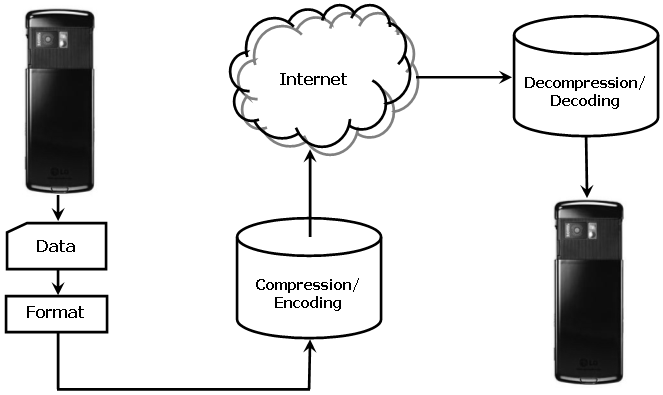
\includegraphics{illus2.png}}
\caption{Verbose Data Formats using Compression/ Decompression}  \label{illus}
\end{center}
\end{figure}

\section{Adding Tables}

\begin{table}[ht]
\caption{Features of XML and YAML}   % title of Table
\label{msgcomm}
\centering                          % used for centering table
%\begin{tabular}{| l | l |}              % centered columns (4 columns)
\begin{tabular}{l  c  l }              % centered columns (4 columns)
\hline                        %inserts double horizontal lines
\cline{1-3}
\hline                        %inserts double horizontal lines
\textbf{Feature} & \textbf{XML} & \textbf{YAML} \\ [0.5ex]   % inserts table heading
\hline                              % inserts single horizontal line
\cline{1-3}
Read/Writeability & Human Readable & Human Readable \\               % inserting body of the table
Data Exchange Among Applications & Applicable & Applicable \\               % inserting body of 
%\cline{1-2} 
Structured Data  & Yes & Yes \\               % inserting body of the table
Intrinsic Support for Data types & No & Yes \\
Verbosity & High & Less \\
Number of APIs    & High &  Less \\
Platform Independence &Yes & Yes \\
Schema Aware &Yes & Yes \\
Built-in Schema &Yes & No \\
Message Level Security Enhancements &Yes & No \\
Schemes for Prevention of Rewriting Attacks &Yes & No \\

\hline                              %inserts single line
\cline{1-3}
\end{tabular}
\end{table}


\section{Adding Equations}

Here is a displayed 
\[\int\frac{d\theta} {1+\theta^2}= 
\tan^{-1}\theta+C\] equation. 

An equivalent way to format the same displayed equation is to spell out the delimiters in words.

Here is a displayed 
\begin{displaymath}\int\frac {d\theta}{1+\theta^2} 
=\tan^{-1} \theta+ C\end{displaymath}
equation. 

A variant of the above is the following.

Here is a displayed 
\begin{equation}\int \frac{d\theta}{1+\theta^2}=
\tan^{-1}\theta+C\end{equation} equation. 

There is a difference between the ``displaymath'' environment and the ``equation'' environment: the latter automatically typesets a formula number. 

What if you want to refer to a numbered equation by number? How do you manage this if the equation number is automatically generated? LaTeX has a simple \label and \ref mechanism for handling symbolic cross references. Here is an example. 

The formula \begin{equation} E=m c^2
\label{Einstein} \end{equation} has passed into popular culture,
but the true significance of the mass-energy
equation~(\ref{Einstein}) is~\ldots 


This paper centers around the humble intention to find out 
whether it is possible to unearth the hitherto unknown information from the 
unstructured text jungle over the WWW, and present it as a structure in 
conformity to the model of Semantic Web.

This reoport is organized as follows: Chapter \ref{pre} outlines the literature survey.
Chapter \ref{rdf} is about the problem definition. In Chapter \ref{desig}, an overview of the proposed 
system is explained. Chapter \ref{res} contains conclusion and a breif discussion about the future work. 
